\documentclass[11pt,a4paper]{article}
\usepackage[margin=23mm]{geometry}
\usepackage[T1]{fontenc}
\usepackage{lmodern,microtype,amsmath,amssymb,booktabs,graphicx,tabularx,array,float}
\usepackage{xcolor,enumitem,fancyhdr}
\usepackage[font=small,labelfont=bf]{caption}
\usepackage[colorlinks=true,linkcolor=teal,citecolor=teal,urlcolor=teal]{hyperref}
\setlength{\parindent}{0pt}
\setlength{\parskip}{5pt}
\setlength{\emergencystretch}{2em}
\setlength{\headheight}{14pt}
\pagestyle{fancy}\fancyhf{}\lhead{COMP9501 Group 13}\rhead{LoRA merging: controlled study}\cfoot{\thepage}
\setlist[itemize]{leftmargin=*,topsep=3pt,itemsep=2pt}
\setlist[enumerate]{leftmargin=*,topsep=3pt,itemsep=2pt}
\newcommand{\method}[1]{\textsc{#1}}
\newcommand{\std}[2]{#1\,$\pm$\,#2}
\newcommand{\AbstractExtension}{The exploratory hidden-response and routing controls give paired effects of -0.0733 native score versus FP32 CE and -6.93 accuracy points versus task-ID routing, respectively.}
\newcommand{\ActivationConclusion}{The paired native-score difference of CE+hidden minus same-precision CE is -0.073280, positive in 0/3 seeds. Against the shuffled-response control the mean difference is +0.020254, positive in 2/3 seeds. The aligned response penalty does not add task-quality benefit over CE in this setting. These descriptive comparisons isolate the selected response-pairing and capacity controls; the sample is too small and the evaluation history too exploratory for a confirmatory claim.}
\newcommand{\RouterConclusion}{The expert router changes mean accuracy relative to task-ID selection by -6.934 percentage points, improving in 0/3 seeds. The GT oracle increases mean accuracy by 10.026 points over task ID. This gap measures bank-level headroom under impossible label access, not a realizable routing gain. Our performance-oriented router fails to realize that headroom and is worse than direct task-ID selection. }
\newcommand{\DiscussionExtension}{The extension results further separate input-response matching from the distribution-preserving shuffle control, and expert identity prediction from actual help or harm relative to task-ID selection.}
\newcommand{\ConclusionExtension}{The direct hidden and task-aware routing extensions report paired changes of -0.0733 native score and -6.93 accuracy points against their respective controls, with the stated exploratory scope.}

\newcommand{\SensitivityVtwo}{Selection chooses zero hidden weight in 2/3 seeds. The selected aligned-grid minus CE native-score difference is +0.007764 on internal final and +0.005542 on cleaned official validation. These are pipeline comparisons with additional selection candidates, not isolated evidence of a unique functional effect.}
\newcommand{\OfficialVtwo}{The retained validation counts are 872, 408, 277, and 1023 for SST-2, MRPC, RTE, and CoLA. The split was previously explored historically; full-tuple overlap filtering does not remove all near duplicates or pretraining contamination.}
\newcommand{\GatesVtwo}{On cleaned official validation, confidence and benefit gates change macro mean accuracy versus task ID by +0.000 and +0.000 percentage points. A selection constraint is not a guarantee on final inputs; the actual help/harm rates and fallback choices determine the interpretation.}
\newcommand{\AbstractVtwo}{A further fixed-grid sensitivity and conservative-routing study evaluates a larger, exact-tuple-cleaned official-validation split. Selected hidden versus CE changes native score by +0.0055; the benefit gate changes macro accuracy versus task ID by +0.00 points, with exploratory scope.}
\newcommand{\ConclusionVtwo}{The larger cleaned-validation follow-up gives selected hidden-minus-CE native change +0.0055 and benefit-gate-minus-task-ID accuracy change +0.00 points. These results describe a selected pipeline under known-task access, not a new blind benchmark or equal-budget mechanism proof.}

\title{Activation-Aware Merging of LoRA Adapters\newline for Multi-Task Learning\\[5pt]
\large A controlled study of similarity, functional objectives, and routing}
\author{COMP9501 Advanced Machine Learning\\Group 13}
\date{11 November 2026}

\begin{document}
\maketitle
\begin{abstract}
Combining task-specific low-rank adaptations can reduce the need to manage distinct weight states, but averaging updates can introduce interference. We investigate whether functional information can predict or mitigate this interference in a small, reproducible multi-task setting. Four Qwen2.5-0.5B adapters are trained on SST-2, MRPC, RTE, and CoLA. A content-grouped five-way protocol separates teacher training, teacher checkpoint selection, merge fitting, merge selection, and final evaluation. Across three training seeds, learned layer-wise coefficients achieve a mean native task score of 0.7132 with cross-entropy (CE), compared with 0.5578 for averaging and 0.6146 for our TIES baseline. Teacher-logit KL reaches 0.6987 and does not outperform the matched-capacity CE control on average. Our initial unit-weight extension tests hidden-response matching, shuffled-response controls, and performance-oriented routing. \AbstractExtension\ \AbstractVtwo\ The study identifies the distinction between source recognition and useful expert selection, and measures routing overhead on an A100. Its contribution is a controlled implementation and analysis of the original hypothesis; it does not establish a new state-of-the-art merging algorithm or robust out-of-domain generalization.
\end{abstract}

\section{Introduction and research questions}
LoRA adapts a pretrained weight matrix using a low-rank update while retaining a shared backbone~\cite{lora}. A collection of task adapters therefore offers a practical multi-task system. A merged model can offer a single backbone weight state, but combining independently trained updates can damage individual task performance. Task Arithmetic, TIES, and DARE provide weight-space approaches to this problem~\cite{ta,ties,dare}.

Our original proposal hypothesized that adapters with similar activations can be merged safely, while conflicting inputs or tasks require dynamic gating. We translate this broad hypothesis into three questions:
\begin{enumerate}
\item \textbf{RQ1:} Does activation similarity reliably predict the performance loss of a task-pair merge?
\item \textbf{RQ2:} Does functional supervision improve a static merge after controlling parameter capacity, optimization, precision, and access to labels?
\item \textbf{RQ3:} Can an input-dependent router select useful experts beyond the directly available task-ID baseline, and what computational cost does this introduce?
\end{enumerate}

We study one small backbone and four binary tasks to permit explicit data and numerical checks. We retain negative results, distinguish exploratory stages, and compare learned coefficients against both fixed weight-space rules and supervised controls. The resulting contribution is a proposal-aligned empirical investigation with reproducible artifacts, an explicit information protocol, and diagnostics of misleading proxy metrics.

The original deployment motivation also requires qualification. Our actual reference system shares one base model and stores four small adapters; it does not duplicate four full backbones. Consequently, a single merged weight state is not automatically a substantial total-storage saving. This distinction matters when judging the practical value of static merging and routing.

\section{Related work and positioning}
Task Arithmetic represents adaptation as displacement from a common pretrained model and combines these task vectors~\cite{ta}. TIES addresses small or conflicting parameter changes through trimming, sign election, and disjoint merging~\cite{ties}. DARE randomly drops and rescales updates before combination~\cite{dare}. We implement explicit variants and use a fixed candidate grid; comparison with these implementations is not a claim to reproduce every official benchmark setting.

Functional information has established precedents. RegMean uses layer-input Gram statistics to match linear-layer responses~\cite{regmean}. AdaMerging learns task-wise or layer-wise coefficients using prediction-entropy adaptation~\cite{adamerge}. KnOTS studies representation alignment in LoRA merging and uses a shared SVD space~\cite{knots}. Hidden-representation supervision also predates this project in knowledge distillation, including FitNets~\cite{fitnets}. These works motivate our tests and constrain novelty claims: layer-wise coefficients, response matching, and low-rank alignment are not inventions of this project.

Our implementation combines a constrained adapter-span parameterization with controlled comparisons of CE, output KL, hidden-response objectives, and routing targets. Unlike the entropy objective of AdaMerging, our coefficient selection uses labels from a declared selection partition. Unlike RegMean and KnOTS, we do not solve full layer-weight regression or perform shared-SVD alignment. Our evidence concerns this implementation and task-aware protocol, not superiority over those complete methods.

\section{Model and merging methods}
\subsection{Adapters, heads, and the task-aware protocol}
For an adapted layer $\ell$, task $t$ supplies
\begin{equation}
 \Delta W_{t,\ell}=\frac{\alpha}{r}B_{t,\ell}A_{t,\ell},\qquad
 W_{t,\ell}=W_{0,\ell}+\Delta W_{t,\ell}.
\end{equation}
We use $r=8$, $\alpha=16$, and the query/value projections of Qwen2.5-0.5B~\cite{qwen}. Each teacher trains its LoRA factors and a task-specific classification head; the pretrained backbone remains frozen. Every evaluation method receives the same known task ID to select the corresponding frozen head. The four binary tasks have different label meanings, so a common output dimension is not a common label space.

We combine materialized $BA$ updates, rather than averaging $A$ and $B$ separately: separate factor averaging introduces cross-adapter products. The sum of four rank-eight updates can have rank up to 32, subject to matrix dimensions and dependencies. Our final static model is a materialized backbone; we do not claim it is a single rank-eight adapter.

\subsection{Static coefficient parameterization}
For each layer, the merge is
\begin{align}
 W_{m,\ell}&=W_{0,\ell}+g\sum_{t=1}^{4}p_{\ell,t}\Delta W_{t,\ell},\\
 p_{\ell,t}&=\operatorname{softmax}(a_\ell)_t,\qquad
 g=0.5+3.5\,\sigma(b).
\end{align}
The layer-wise variant stores $24\times4+1=97$ trainable scalars; a global vector stores five. Softmax introduces a shift redundancy, so these are tensor parameter counts, not independent degrees of freedom. Within a layer, query and value updates share the task mixture. Base weights, adapter factors, and task heads remain frozen during coefficient fitting.

The regularizer penalizes deviation from uniform mixture weights and from gain two:
\begin{equation}
 R=\frac{1}{L}\sum_\ell\sum_t(p_{\ell,t}-1/4)^2+
       \log^2(g/2).
\end{equation}
Its weight is 0.01. Fitting evaluates the exact low-rank response of the weighted update. Deployment materializes the selected $\Delta W$ into one backbone.

\subsection{CE and teacher-output KL}
The CE control optimizes ground-truth classification loss. The output-matching variant minimizes
\begin{equation}
 \mathcal L_{\rm KL}=T^2\,D_{\rm KL}\!\left(
 \operatorname{softmax}(z_t/T)\,\Vert\,
 \operatorname{softmax}(z_m/T)\right),\quad T=2,
\end{equation}
where $z_t$ is the frozen individual teacher's output for its own task. Both variants use the same coefficient capacity, initialization, update count, sample order, and label-based checkpoint-selection access. KL does not use fit labels in its gradient target, but teacher training and merge selection use labels. The complete pipeline is therefore supervised. Output KL also does not directly test an intermediate-activation similarity hypothesis.

\subsection{Task-conditioned local-response prototype}
Our earlier static prototype uses linear adapter responses to connect the proposal's similarity idea with a fitting objective. On task-$t$ calibration inputs, we collect each adapted module's input $x_\ell^{(t)}$ along the individual teacher's path and compute every adapter response $u_{j,\ell}=\Delta W_{j,\ell}x_\ell^{(t)}$. A constrained quadratic fit minimizes the mismatch between $\sum_j p_{\ell,j}u_{j,\ell}$ and the own-teacher response $u_{t,\ell}$, with simplex weights and optional shrinkage toward uniform. Response Gram matrices are normalized by output dimension and valid-token count; the global variant additionally normalizes block traces. Gain is selected separately.

This is a response-statistics method restricted to the adapter span, related to the output-preservation motivation of RegMean. It is not RegMean's full weight-matrix solution. Using identical inputs and equally weighted targets also admits uniform averaging as an optimum, so task-conditioned paths provide the additional information. Lowering a local quadratic surrogate does not guarantee the behavior of the nonlinear materialized network. We retain this prototype as exploratory protocol-v2 evidence.

\newpage
\subsection{Direct hidden-response objectives and controls}
Let $h_t(x)$ be the attention-mask token mean of the final hidden layer, and let $h_0(x)$ be the corresponding base response. Define $d_t=h_t-h_0$ and $d_m=h_m-h_0$. The new hidden objective is
\begin{equation}
 \mathcal L_H=\frac{1}{N}\sum_i
 \frac{D^{-1}\sum_j(d_{m,ij}-d_{t,ij})^2}
 {\max\{D^{-1}\sum_j d_{t,ij}^2,10^{-4}\}}.
\end{equation}
Subtracting the same base cancels in the numerator: the distinctive normalization uses teacher update energy, not a new distance identity. This mean-pooling proxy also differs from the model's native classification pooling, so small hidden loss does not guarantee preserved class decisions.

We compare five FP32 profiles: layer CE, layer hidden-only, layer CE+$H$, layer CE+shuffled $H$, and global hidden-only. The combined hidden weight is fixed at one. The shuffled control applies a fixed within-task derangement to teacher deltas: it retains the target set while destroying same-input correspondence. This tests whether pairing carries information beyond the response distribution. It does not remove every source-style cue. The FP32 CE control isolates loss changes within the extension; historical BF16 CE/KL rows remain separately identified.

\subsection{Input-dependent routing and oracle analysis}
A source router predicts the input dataset using frozen base mean features. Our extension also fits a performance-oriented router. For each fit input with label $y$, its target is the expert minimizing ground-truth negative log-likelihood under the known task head. Its features concatenate standardized base responses and the already available task one-hot vector. This fitting requires fit labels and offline evaluation of all experts.

Both routers select logistic-regression $C\in\{0.1,1,10\}$ using the same merge-selection task metric. We compare them with direct task-ID selection and seeded random routing. An analysis-only oracle selects the final-set expert with highest true-class probability. It gives an accuracy ceiling for this bank/head protocol, using final labels, and cannot be deployed. Agreement with its minimum-NLL expert identity is distinct from task accuracy.


\subsection{Loss-weight sensitivity and conservative gates}
The unit hidden-loss weight is a fixed design choice, not an established optimum. A follow-up grid uses $\lambda\in\{0,0.01,0.1,1\}$ with the same 97 scalars, FP32, initialization, update count and sampled examples. We reuse the completed zero (CE) and unit-weight endpoints and fit the two intermediate weights for aligned and shuffled targets. Each lambda first selects its step on the original merge-selection role; the grid then selects lambda by that role's native metric, preferring smaller lambda on ties. Aligned and shuffled grids have equal candidate budgets, but both offer more selection candidates than the single CE trajectory.

A confidence gate reuses the frozen expert-ID classifier and switches only above maximum-probability thresholds $0,0.5,0.7,0.9$, or chooses always-own. A benefit gate instead fits four Ridge regressions to fit-set correctness differences,
\begin{equation}
 y_j(x)=\mathbf{1}[\hat y_j(x)=y]-\mathbf{1}[\hat y_{\rm own}(x)=y].
\end{equation}
Its inputs are standardized base features and known task one-hot. Ridge strengths are $1,100,10000$; predicted-gain thresholds are $0,0.02,0.05,0.1$. The own expert has fixed reference gain zero. These are uncalibrated regression scores, not probabilities of benefit. Fitting uses class labels and all experts' offline predictions; its capacity and information budget differ from static coefficient fitting.

Both gate families include always-own. Eligible selection candidates must have native score and macro accuracy at least task ID, and worst-task accuracy no more than 0.01 lower. We then maximize native score, macro accuracy, and finally minimize switching; remaining ties retain the baseline. These constraints concern selection data only and do not guarantee final safety. Serialized scalers and coefficients are reloaded and checked against the in-memory routes. An always-own choice can bypass feature extraction at serving, but represents rejection of the new router rather than a new routing gain.

The combiner uses only selection fields to choose lambda and gates, then writes choices before reading cached final prediction arrays or loading official validation. Earlier final metrics already coexist in run files and had informed this follow-up design; this order does not create a pristine-test claim.

\subsection{A larger, content-filtered evaluation split}
We additionally evaluate pinned GLUE official validation after selection is locked. We remove normalized complete text tuples found in \emph{any original training example} across the four tasks, then deduplicate tuples within each validation task. Filtering uses text only, not labels. Exact IDs, content hashes, fingerprints and removal counts are recorded. Near duplicates, sentence reuse within different pairs and pretraining contamination remain possible. Official validation was explored historically with earlier teachers, so this is a larger separate-split check, not a new blind benchmark or proof of OOD robustness.

The locked comparison includes task ID, source/expert routers, the two gates, GT oracle, FP32 CE, selected aligned/shuffled grids, and the original v3 selection-locked Average/TA/TIES/DARE variants. Tasks have different retained sample counts: accuracy is macro-averaged over tasks, whereas switching fraction counts individual inputs. Three teacher seeds still give three replications; repeated coefficient fits do not increase this number.

\section{Experimental protocol}
\subsection{Data and information boundaries}
We use SST-2, MRPC, RTE, and CoLA from GLUE~\cite{glue}. Protocol v3 splits the original training data into five content-grouped roles. Normalized complete field tuples receive a fixed hash-based role independent of class labels; duplicates share a role, including across tasks. One representative per normalized tuple is retained. Dataset revision, source fingerprint, IDs, and manifest SHA are saved.

\begin{table}[H]\centering\small
\caption{Protocol v3 sample counts per task. Final is an internal partition of original train, not official GLUE validation.}
\begin{tabular}{lrrrrr}\toprule
Task & Train & Teacher select & Merge fit & Merge select & Final\\\midrule
SST-2 &4096&128&128&128&256\\
MRPC &2391&128&128&128&256\\
RTE &1571&128&128&128&256\\
CoLA &4096&128&128&128&256\\\bottomrule
\end{tabular}\end{table}

All 12 teachers are freshly trained under these boundaries. Re-splitting an old calibration pool would not undo prior teacher checkpoint selection, so old teachers are not reused for v3. Exact-tuple grouping does not remove near duplicates, repeated individual sentences within different pairs, or possible pretraining contamination. Earlier GLUE exploration also informed the research. The new hidden/routing extension was designed after seeing v3 final results and is explicitly exploratory; per-run fit/select separation does not restore pristine-test status.

\subsection{Training, selection, and comparators}
Teachers use three epochs, batch 16, maximum length 128, LoRA dropout 0.05, adapter learning rate $2\cdot10^{-4}$ and head rate $10^{-3}$. Teacher selection minimizes loss on its dedicated role. Training seeds are 42, 43, and 44; the pretrained backbone and common head-initialization seed are fixed. These seeds quantify some training variability on one shared partition, not independent dataset replications.

Coefficient profiles use Adam, 120 updates, batch eight, learning rate 0.03, and checkpoint candidates $\{0,30,60,90,120\}$. Step zero is included; ties keep the earlier step. Selection maximizes the macro mean of SST-2/RTE accuracy, MRPC $(\mathrm{accuracy}+F_1)/2$, and CoLA MCC. We call this the \emph{native task score}; it is not the full official GLUE score. We additionally report mean accuracy, worst-task accuracy, and the drop relative to the same-seed individual teacher.

The extension uses the allocated NVIDIA L4 after A100 availability could not be obtained. Its new FP32 controls share the same device and precision. Historical v3 teacher training, BF16 coefficient fits, and the separate serving-cost benchmark used A100. We keep these stages distinct and check restored teacher task-ID performance against the saved reference; any numerical runtime difference is recorded rather than treated as a new training outcome.

Weight-space comparators use a fixed 17-candidate grid: averaging; TA scales 0.25/0.5/1; per-matrix TIES retention 0.2/0.5 and scale 0.5/1; DARE retention 0.9/0.5/0.1 and TA scale 0.25/0.5/1. DARE mask seed stays 42. Four-task averaging equals TA scale 0.25. Selection samples are shared, but candidate counts, fit supervision, and optimization cost differ; this is not an equal-total-information or equal-compute comparison.

Each run writes selected choices before loading its final role. The extension preserves this execution order while disclosing prior final-set inspection. All tables report three-seed means and sample standard deviations. With $n=3$, we show paired outcomes and avoid significance claims.

\section{Results}
\subsection{RQ1: similarity is an unstable merge-safety proxy}
Our earlier protocol-v2 diagnostic evaluated the six equal-weight pairs of four tasks. Spearman correlations between delta-activation cosine and mean pair accuracy loss were $-0.6571$, $-0.4857$, and $+0.0857$ across three training seeds. Delta similarity was more negatively associated than raw similarity in only one seed. Six pairs share adapters, so the 18 pair/seed observations are not independent experiments.

This exploratory evidence does not establish a reliable safety threshold. Raw similarity can be dominated by the common pretrained model, while subtracting a base response makes the signal more update-specific without ensuring that it predicts nonlinear merged-model quality. Protocol-v2 pair diagnostics and protocol-v3 final scores are presented as separate stages rather than pooled into one confirmatory result.

The protocol-v2 local-response fit similarly failed to improve its uniform reference: global/layer native means were approximately 0.6226/0.6227, against 0.6365 for the selected uniform gain. This motivates testing end-to-end objectives and their controls rather than treating response-Gram optimization as sufficient evidence of a useful merge.

\subsection{Protocol-v3 main comparison}
\begin{table}[H]\centering\small
\caption{Frozen protocol-v3 results. Three training seeds; mean and sample SD. Native score is the macro task-specific metric, not official GLUE.}
\begin{tabular}{lrrr}\toprule
Method & Native score & Mean accuracy & Worst accuracy\\\midrule
Individual & 0.7695 $\pm$ 0.0114 & 0.8252 $\pm$ 0.0083 & 0.7487 $\pm$ 0.0137\\
Average & 0.5578 $\pm$ 0.0246 & 0.7080 $\pm$ 0.0068 & 0.5430 $\pm$ 0.0377\\
Task Arithmetic & 0.5954 $\pm$ 0.0211 & 0.7152 $\pm$ 0.0132 & 0.5872 $\pm$ 0.0148\\
TIES (our variant) & 0.6146 $\pm$ 0.0240 & 0.7152 $\pm$ 0.0096 & 0.5378 $\pm$ 0.0293\\
DARE+TA & 0.6065 $\pm$ 0.0287 & 0.7077 $\pm$ 0.0131 & 0.5443 $\pm$ 0.0482\\
Uniform, selected gain & 0.5889 $\pm$ 0.0256 & 0.7223 $\pm$ 0.0069 & 0.5768 $\pm$ 0.0328\\
Layer CE (v3 BF16 fit) & 0.7132 $\pm$ 0.0225 & 0.7848 $\pm$ 0.0031 & 0.6875 $\pm$ 0.0141\\
Layer KL (v3 BF16 fit) & 0.6987 $\pm$ 0.0080 & 0.7829 $\pm$ 0.0073 & 0.6719 $\pm$ 0.0273\\
\bottomrule\end{tabular}\end{table}

The v3 results show substantial interference under averaging. Learned layer coefficients improve the fixed weight-space grid, but the matched-capacity CE control exceeds teacher-output KL in mean native task score. Their paired KL-minus-CE differences are $+0.014052$, $-0.045911$, and $-0.011545$, averaging $-0.014468$. Thus the observed improvement over weight rules cannot be uniquely assigned to the teacher-output target.

Individual remains the available task-aware quality reference. CE mean accuracy is 0.7848 versus 0.8252 for individual; worst-task accuracy is 0.6875 versus 0.7487. CE's fit labels and additional optimization also distinguish it from the weight rules, so improvement over TIES is an empirical pipeline comparison rather than a pure capacity-independent activation effect.

\begin{figure}[H]\centering
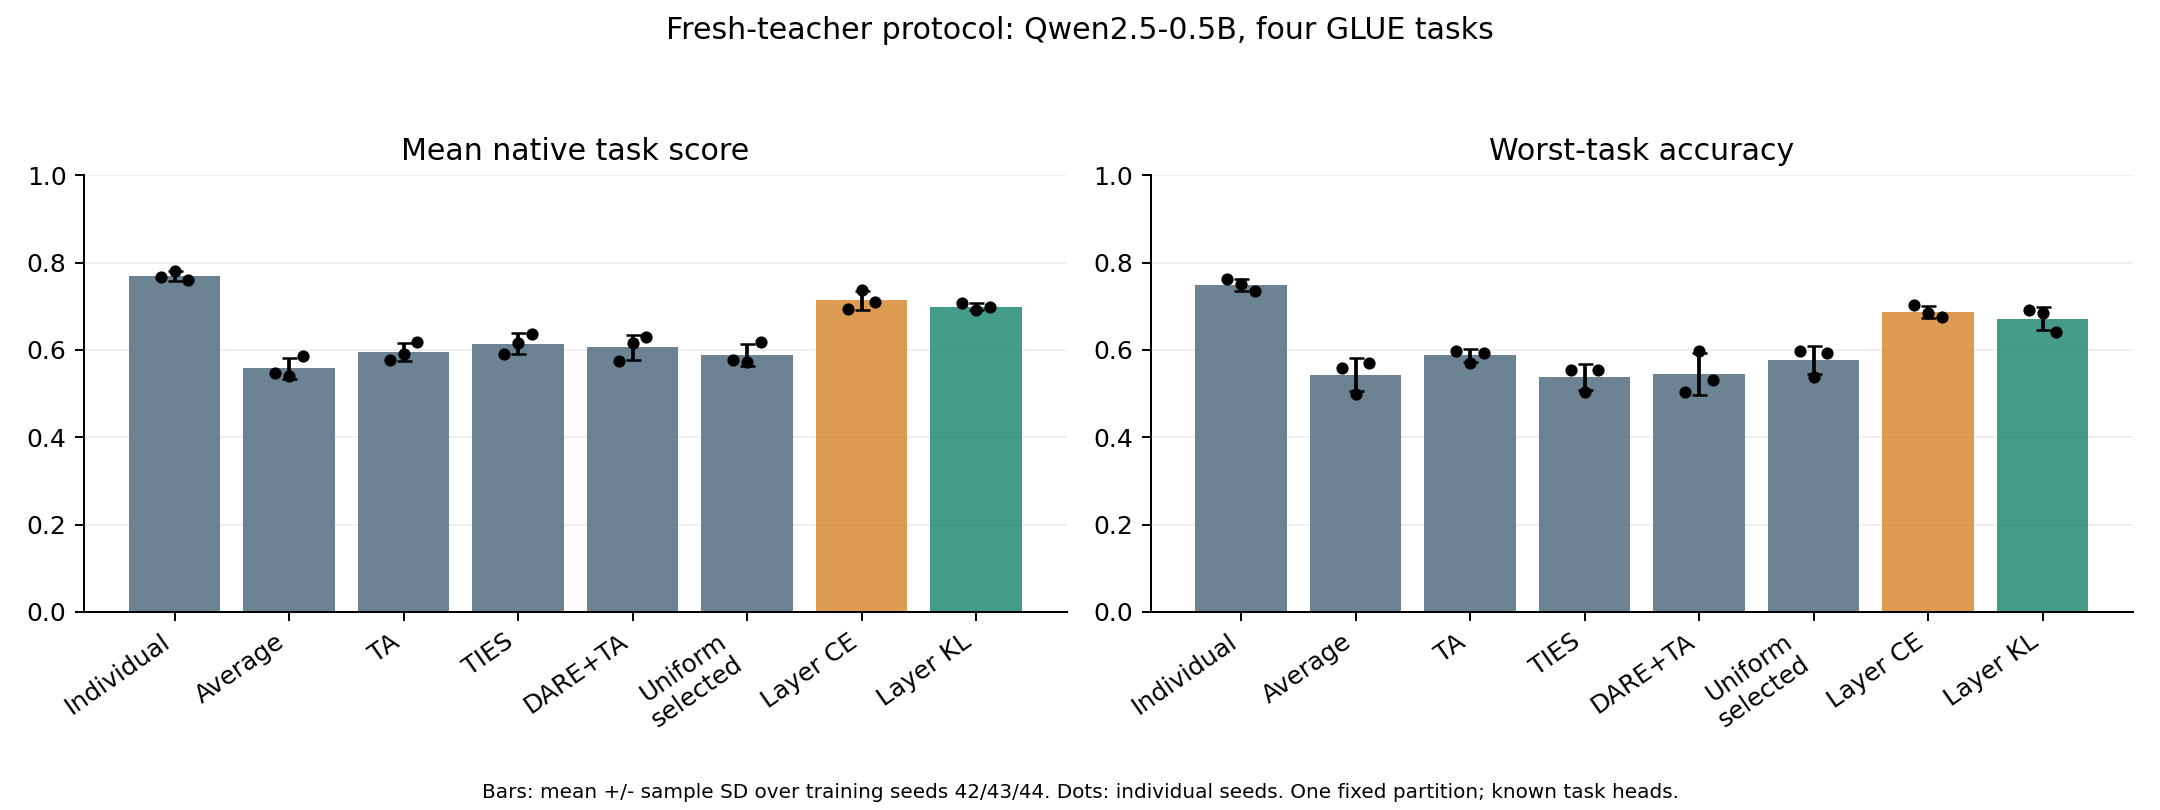
\includegraphics[width=\linewidth]{../artifacts/independent-v3-2026-11-09/main-comparison.png}
\caption{Frozen v3 baseline study: means, sample SD, and individual training seeds. Native metric definitions differ by task; worst-task accuracy is computed per seed before aggregation.}
\end{figure}

\subsection{RQ2: direct activation controls}
\begin{table}[H]\centering\small
\caption{Exploratory direct-activation controls. All FP32. Layer methods have 97 scalars; global has five.}
\begin{tabular}{lrrr}\toprule
Method & Native score & Mean accuracy & Worst accuracy\\\midrule
Layer CE (FP32) & 0.7130 $\pm$ 0.0211 & 0.7861 $\pm$ 0.0029 & 0.6901 $\pm$ 0.0137\\
Layer hidden & 0.5901 $\pm$ 0.0259 & 0.7285 $\pm$ 0.0010 & 0.5820 $\pm$ 0.0170\\
Layer CE + hidden & 0.6397 $\pm$ 0.0281 & 0.7643 $\pm$ 0.0182 & 0.6927 $\pm$ 0.0407\\
Layer CE + shuffled & 0.6195 $\pm$ 0.0056 & 0.7510 $\pm$ 0.0195 & 0.6641 $\pm$ 0.0629\\
Global hidden & 0.5841 $\pm$ 0.0297 & 0.7298 $\pm$ 0.0166 & 0.6055 $\pm$ 0.0768\\
\bottomrule\end{tabular}\end{table}

\ActivationConclusion

\begin{figure}[H]\centering
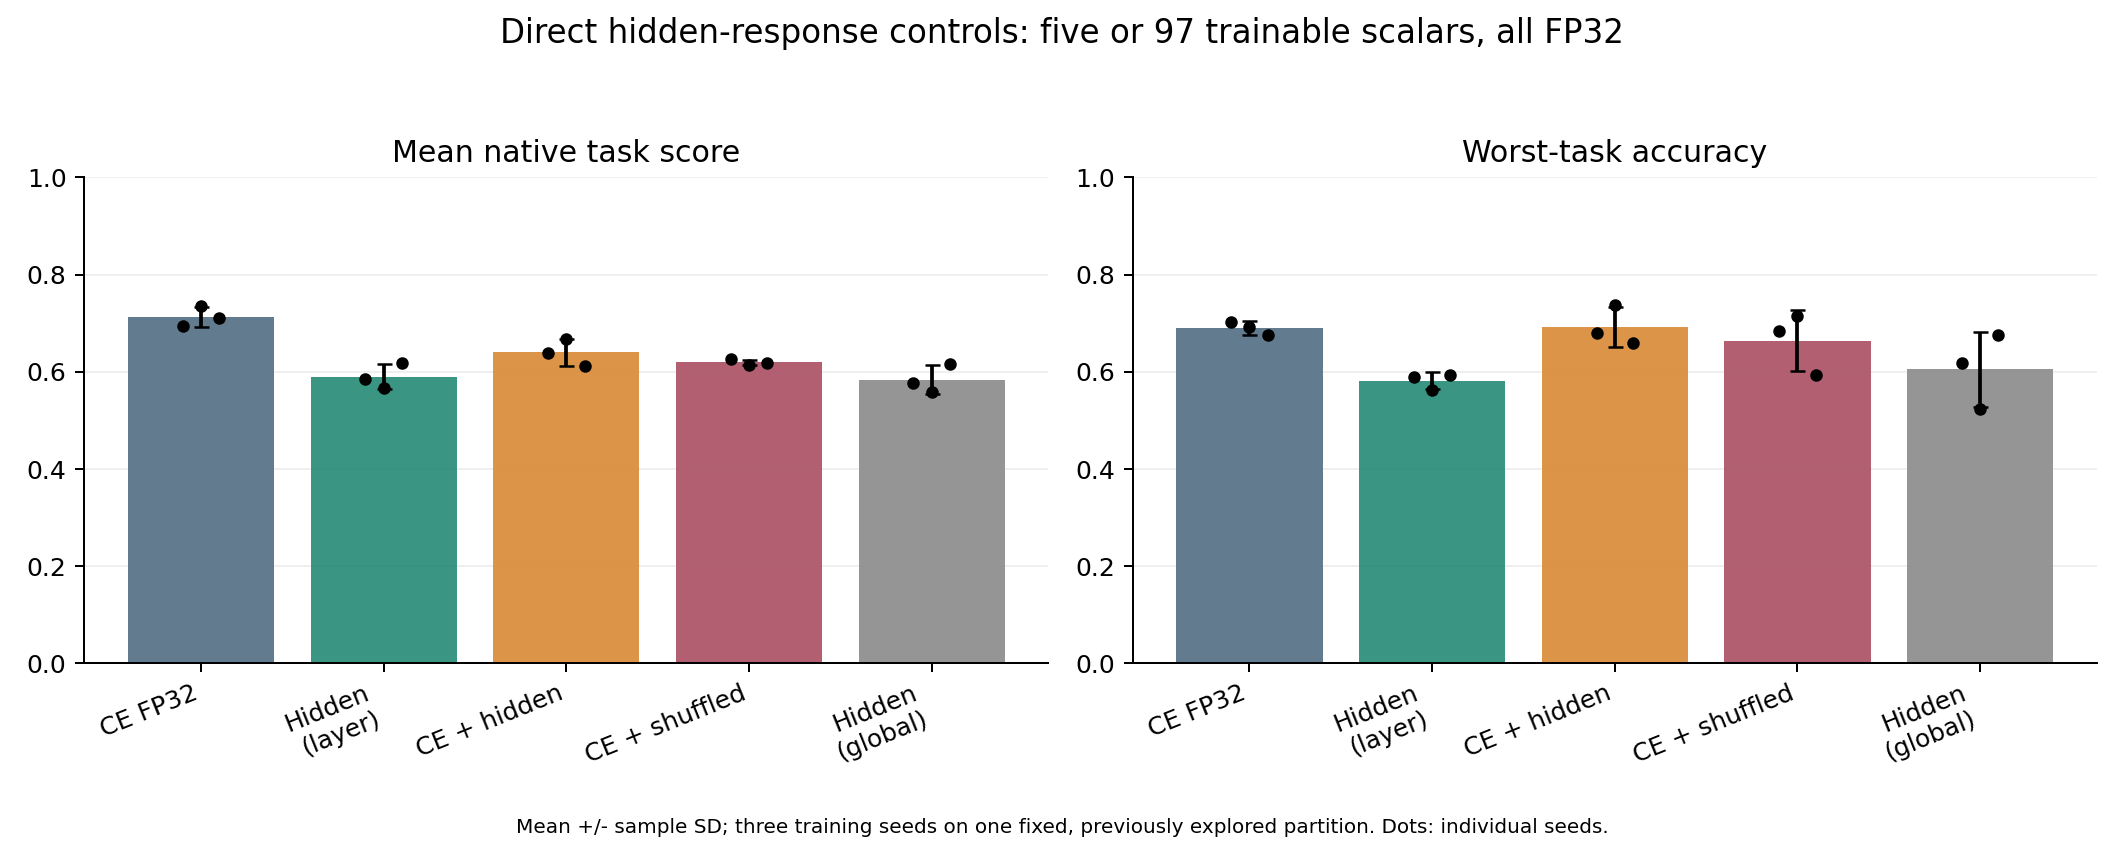
\includegraphics[width=\linewidth]{../artifacts/activation-strengthening-2026-11-11/activation-controls.png}
\caption{Exploratory FP32 activation controls. CE+$H$ and CE+shuffled $H$ share parameter count and update schedule. Global hidden-only has five scalars; the layer variants have 97. The fixed v3 final partition had already informed this extension's design.}
\end{figure}

The selected coefficient checkpoints are also evaluated on the aligned hidden-fit objective. This is a diagnostic, not an additional selection criterion. Reduction of a response surrogate is meaningful only alongside task quality and the shuffled control; optimizing a representation proxy can preserve irrelevant features or conflict with classification requirements.


\subsection{Follow-up: is unit hidden weight too strong?}
\begin{table}[H]\centering\small
\caption{Fixed lambda sensitivity. Same precision/capacity; three teacher seeds. Zero is CE. Lambda grid increases selection budget.}
\begin{tabular}{lrrrr}\toprule
$\lambda$ & Aligned select & Shuffle select & Aligned final & Shuffle final\\\midrule
0.0 & 0.6870 $\pm$ 0.0444 & 0.6870 $\pm$ 0.0444 & 0.7130 $\pm$ 0.0211 & 0.7130 $\pm$ 0.0211\\
0.01 & 0.6835 $\pm$ 0.0346 & 0.6832 $\pm$ 0.0356 & 0.7182 $\pm$ 0.0158 & 0.7199 $\pm$ 0.0141\\
0.1 & 0.6778 $\pm$ 0.0345 & 0.6752 $\pm$ 0.0358 & 0.7029 $\pm$ 0.0363 & 0.6854 $\pm$ 0.0436\\
1.0 & 0.6109 $\pm$ 0.0097 & 0.6051 $\pm$ 0.0194 & 0.6397 $\pm$ 0.0281 & 0.6195 $\pm$ 0.0056\\
\bottomrule\end{tabular}\end{table}

\SensitivityVtwo

Both families select $\lambda=0.01$ for seed 42 and CE ($\lambda=0$) for seeds 43 and 44. On cleaned official validation, the shuffled grid is descriptively slightly higher than the aligned grid (0.7107 versus 0.7106). Thus the small grid-selected gain over CE does not isolate a benefit of correct input-response correspondence; two seeds use no hidden target at all. Generic regularization or additional selection opportunities are possible explanations, not mechanisms established by these data.
\begin{figure}[H]\centering
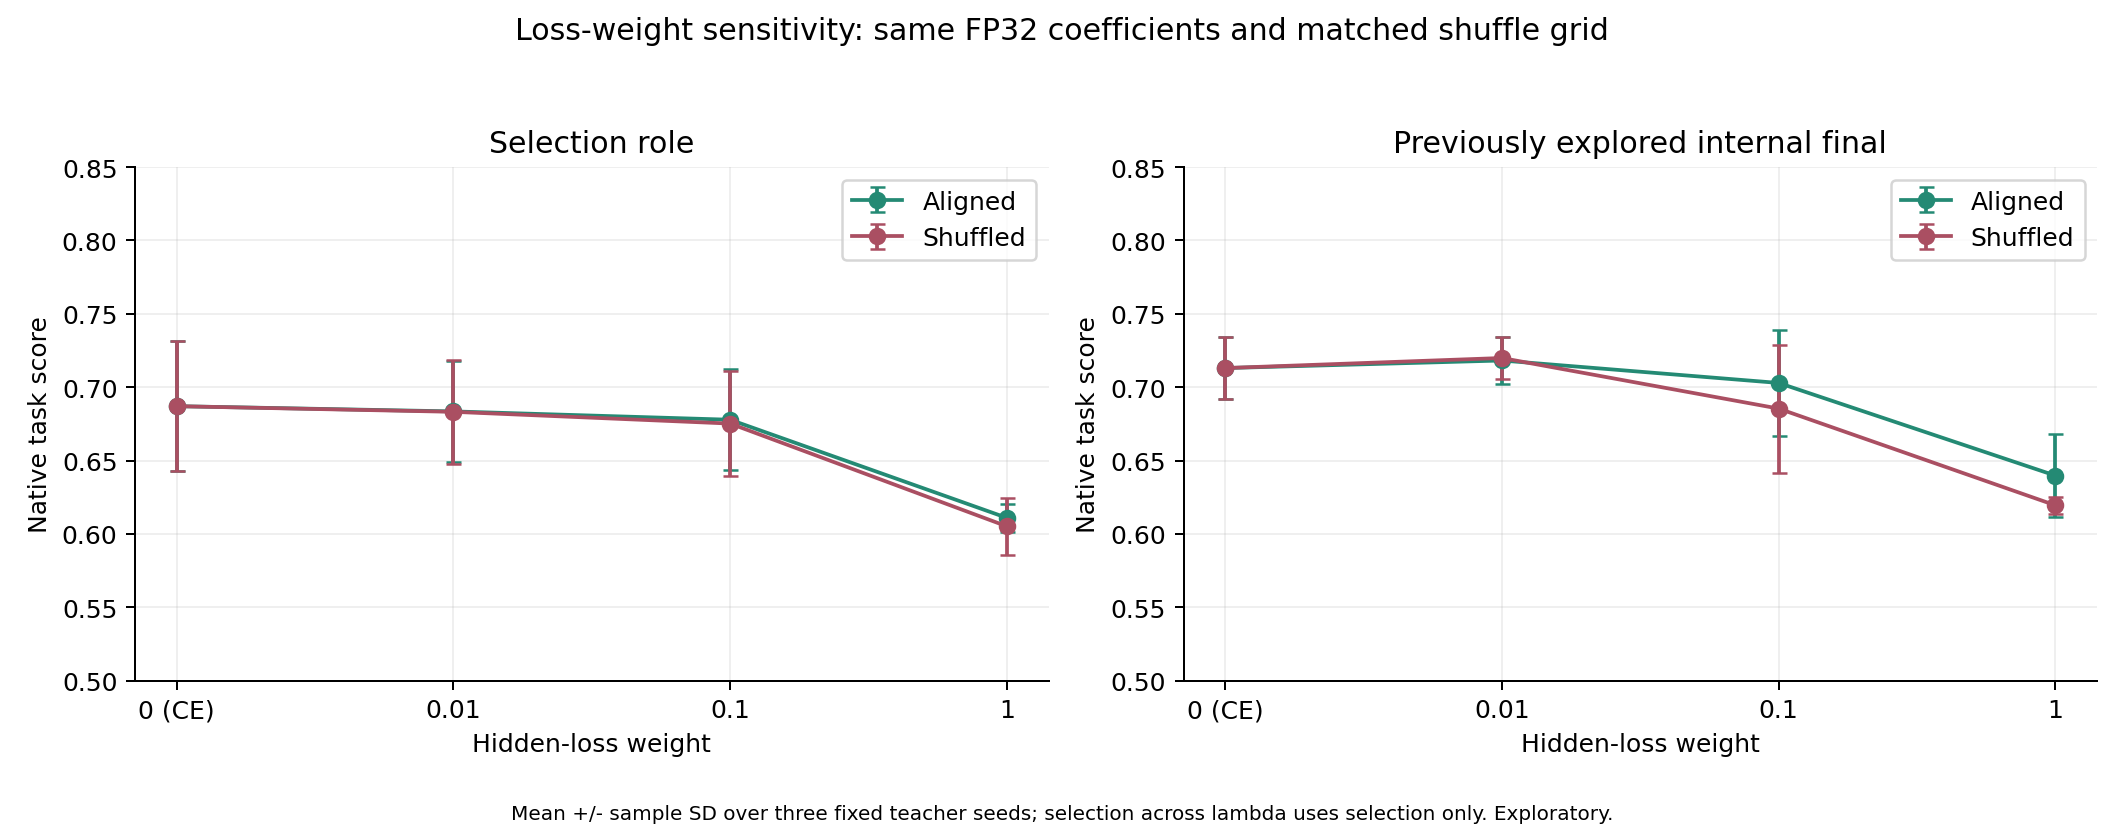
\includegraphics[width=\linewidth]{../artifacts/robustness-v2-2026-11-11/lambda-sensitivity.png}
\caption{Predeclared lambda sensitivity. Selection and previously explored internal-final metrics are shown separately. Aligned and shuffled grids share budgets; zero is the CE reference, not a functional-method improvement.}
\end{figure}

\subsection{RQ3: routing useful experts}
\begin{table}[H]\centering\small
\caption{Exploratory task-aware routing. Oracle is a GT-assisted accuracy ceiling; native scores are not claimed to be upper bounds.}
\begin{tabular}{lrrr}\toprule
Method & Native score & Mean accuracy & Worst accuracy\\\midrule
Task ID / own expert & 0.7695 $\pm$ 0.0114 & 0.8252 $\pm$ 0.0083 & 0.7487 $\pm$ 0.0137\\
Source router & 0.7683 $\pm$ 0.0119 & 0.8232 $\pm$ 0.0083 & 0.7448 $\pm$ 0.0137\\
Expert router & 0.6559 $\pm$ 0.0098 & 0.7559 $\pm$ 0.0051 & 0.6497 $\pm$ 0.0239\\
Random & 0.5787 $\pm$ 0.0298 & 0.6875 $\pm$ 0.0220 & 0.5781 $\pm$ 0.0295\\
Oracle (final GT) & 0.8974 $\pm$ 0.0028 & 0.9255 $\pm$ 0.0025 & 0.8685 $\pm$ 0.0090\\
\bottomrule\end{tabular}\end{table}

\RouterConclusion

\begin{figure}[H]\centering
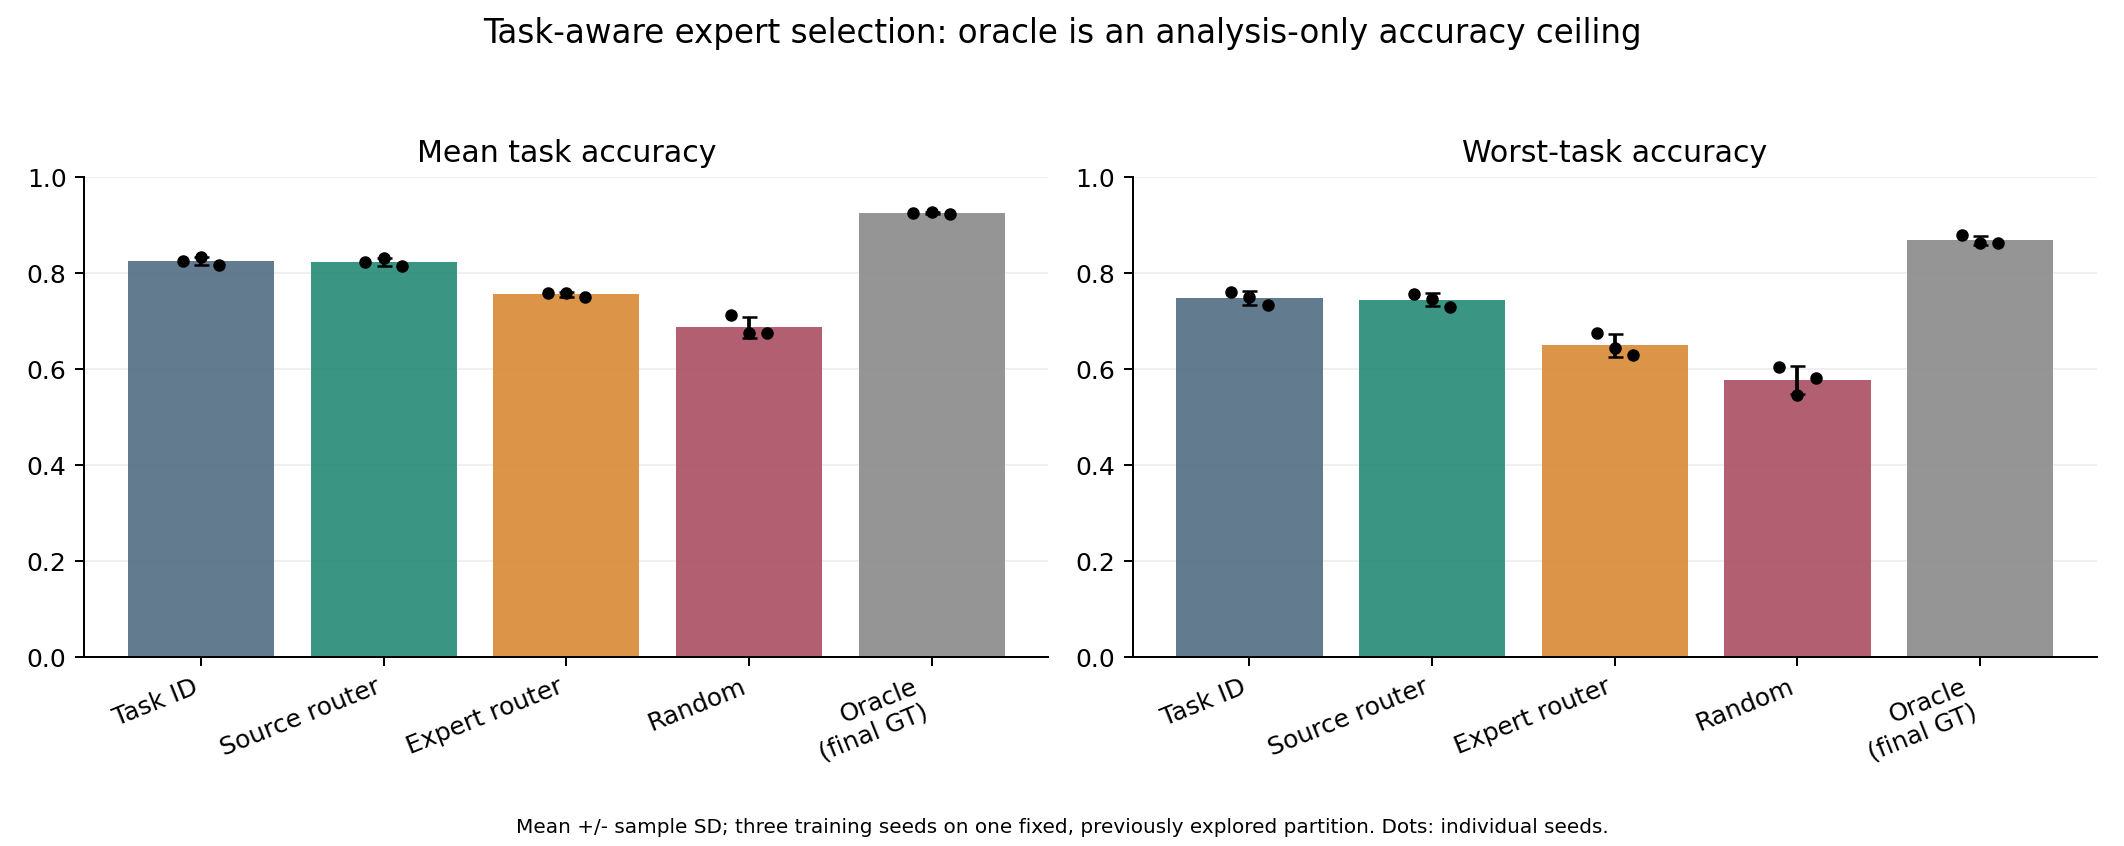
\includegraphics[width=\linewidth]{../artifacts/activation-strengthening-2026-11-11/routing-controls.png}
\caption{Task-aware routing analysis. Oracle uses final labels and is an accuracy ceiling, not an achievable serving result. Expert caches are used for offline analysis; their evaluation time is not a measurement of a deployed router.}
\end{figure}

We report the fractions of inputs helped and harmed relative to the own-task expert. Their difference equals the accuracy change, providing a direct interpretation of routing decisions. Source accuracy describes how often a route agrees with task identity; it does not establish that the choice improves prediction. The expert router additionally uses fit class labels and known task information, which must be included in its information budget.


\subsection{Follow-up: conservative gates and cleaned official validation}
\OfficialVtwo
\begin{table}[H]\centering\small
\caption{Locked methods on cleaned official GLUE validation. Prior historical exploration remains disclosed; oracle uses final GT.}
\begin{tabular}{lrrr}\toprule
Method & Native score & Mean accuracy & Worst accuracy\\\midrule
Individual / task ID & 0.7618 $\pm$ 0.0153 & 0.8225 $\pm$ 0.0164 & 0.7353 $\pm$ 0.0623\\
Average & 0.5738 $\pm$ 0.0178 & 0.7111 $\pm$ 0.0033 & 0.5391 $\pm$ 0.0205\\
Task Arithmetic & 0.5874 $\pm$ 0.0170 & 0.7025 $\pm$ 0.0063 & 0.5571 $\pm$ 0.0149\\
TIES & 0.6007 $\pm$ 0.0095 & 0.7024 $\pm$ 0.0066 & 0.5223 $\pm$ 0.0290\\
DARE+TA & 0.5952 $\pm$ 0.0277 & 0.6971 $\pm$ 0.0120 & 0.5387 $\pm$ 0.0578\\
CE FP32 & 0.7050 $\pm$ 0.0220 & 0.7803 $\pm$ 0.0174 & 0.6750 $\pm$ 0.0719\\
Selected aligned H & 0.7106 $\pm$ 0.0207 & 0.7807 $\pm$ 0.0179 & 0.6703 $\pm$ 0.0662\\
Selected shuffled H & 0.7107 $\pm$ 0.0208 & 0.7806 $\pm$ 0.0177 & 0.6703 $\pm$ 0.0662\\
Source router & 0.7552 $\pm$ 0.0137 & 0.8178 $\pm$ 0.0153 & 0.7316 $\pm$ 0.0646\\
Expert router & 0.6571 $\pm$ 0.0219 & 0.7565 $\pm$ 0.0167 & 0.6462 $\pm$ 0.0407\\
Confidence gate & 0.7618 $\pm$ 0.0153 & 0.8225 $\pm$ 0.0164 & 0.7353 $\pm$ 0.0623\\
Benefit gate & 0.7618 $\pm$ 0.0153 & 0.8225 $\pm$ 0.0164 & 0.7353 $\pm$ 0.0623\\
Oracle (final GT) & 0.8819 $\pm$ 0.0165 & 0.9150 $\pm$ 0.0146 & 0.8437 $\pm$ 0.0503\\
\bottomrule\end{tabular}\end{table}

\GatesVtwo

Both gate families select always-own in all three seeds. The zero final gain records the selection and tie rules preferring the available baseline over learned alternatives. Some strongly regularized benefit candidates satisfy the selection floors but tie the reference; fewer switches or the baseline tie preference decides between them. This is not successful learning of useful switches. It avoids the original expert router's harms by retaining the existing task-ID reference. This is not a new routing accuracy advantage.
\begin{figure}[H]\centering
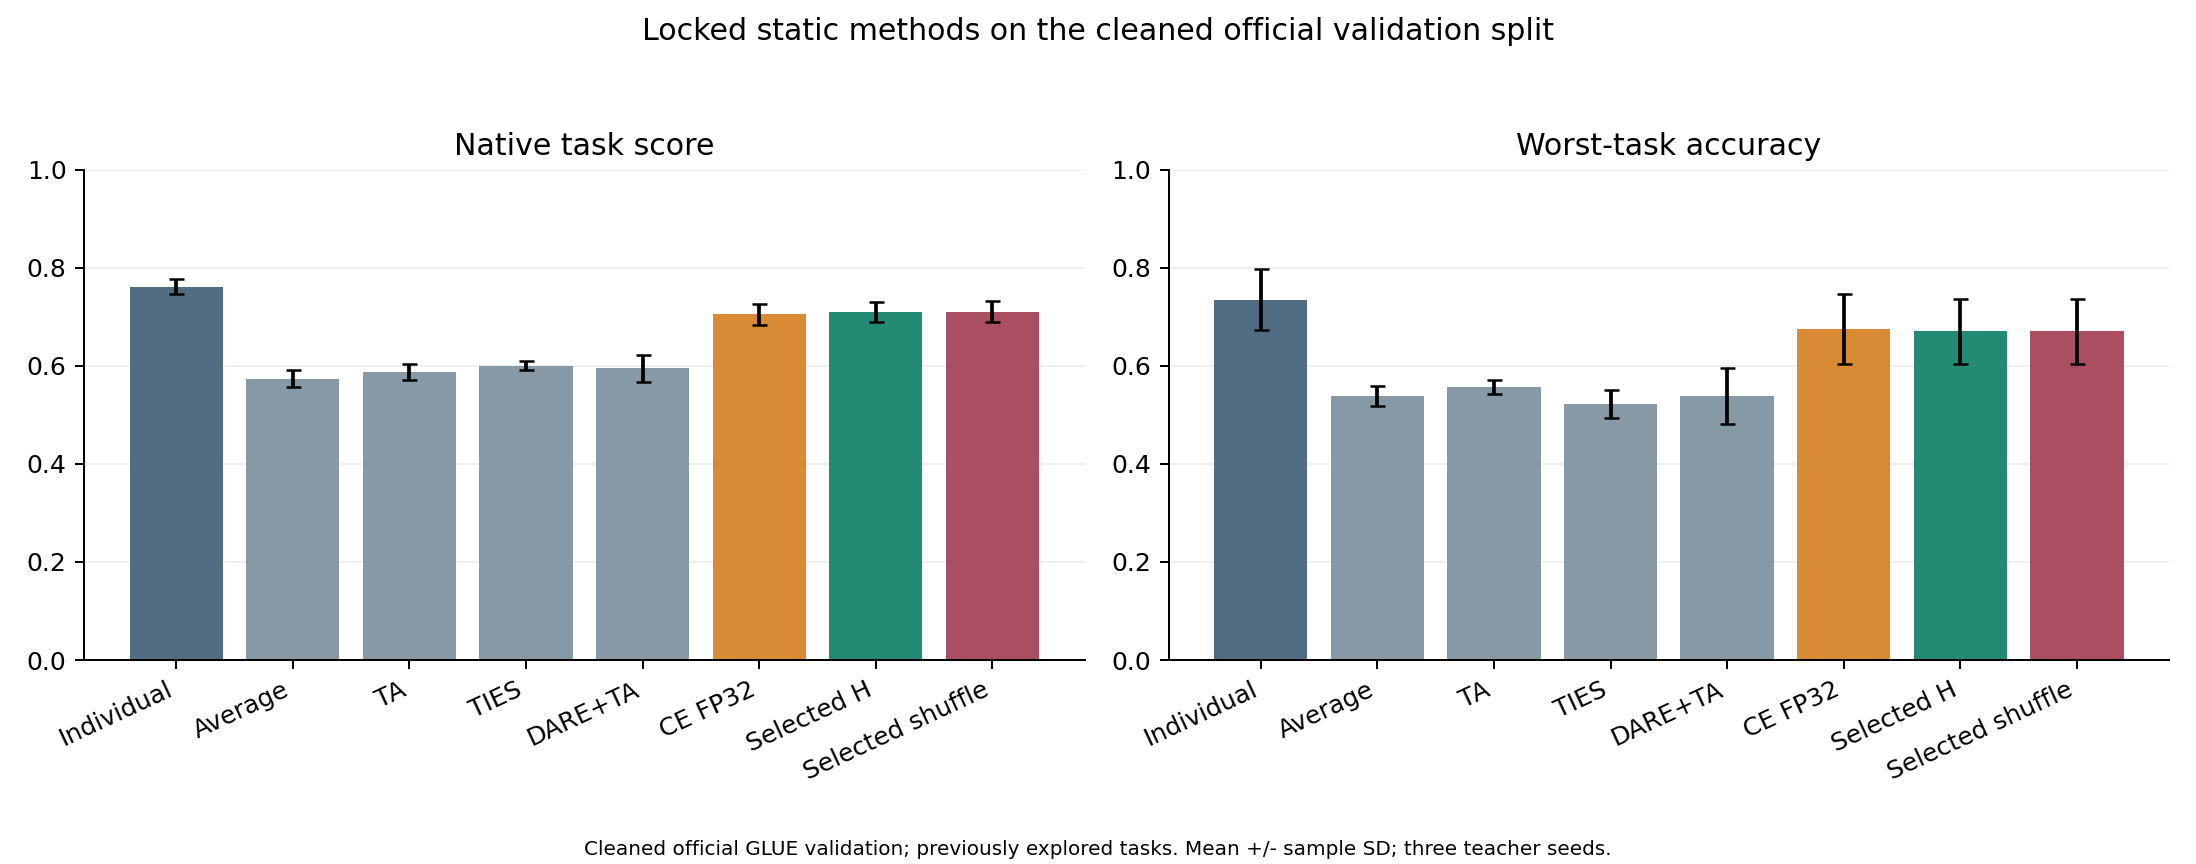
\includegraphics[width=\linewidth]{../artifacts/robustness-v2-2026-11-11/official-static.png}
\caption{Locked static pipelines on cleaned official validation. Extra lambda candidates change the tuning budget. All methods use the known task head; tasks and the official split were historically explored.}
\end{figure}
\begin{figure}[H]\centering
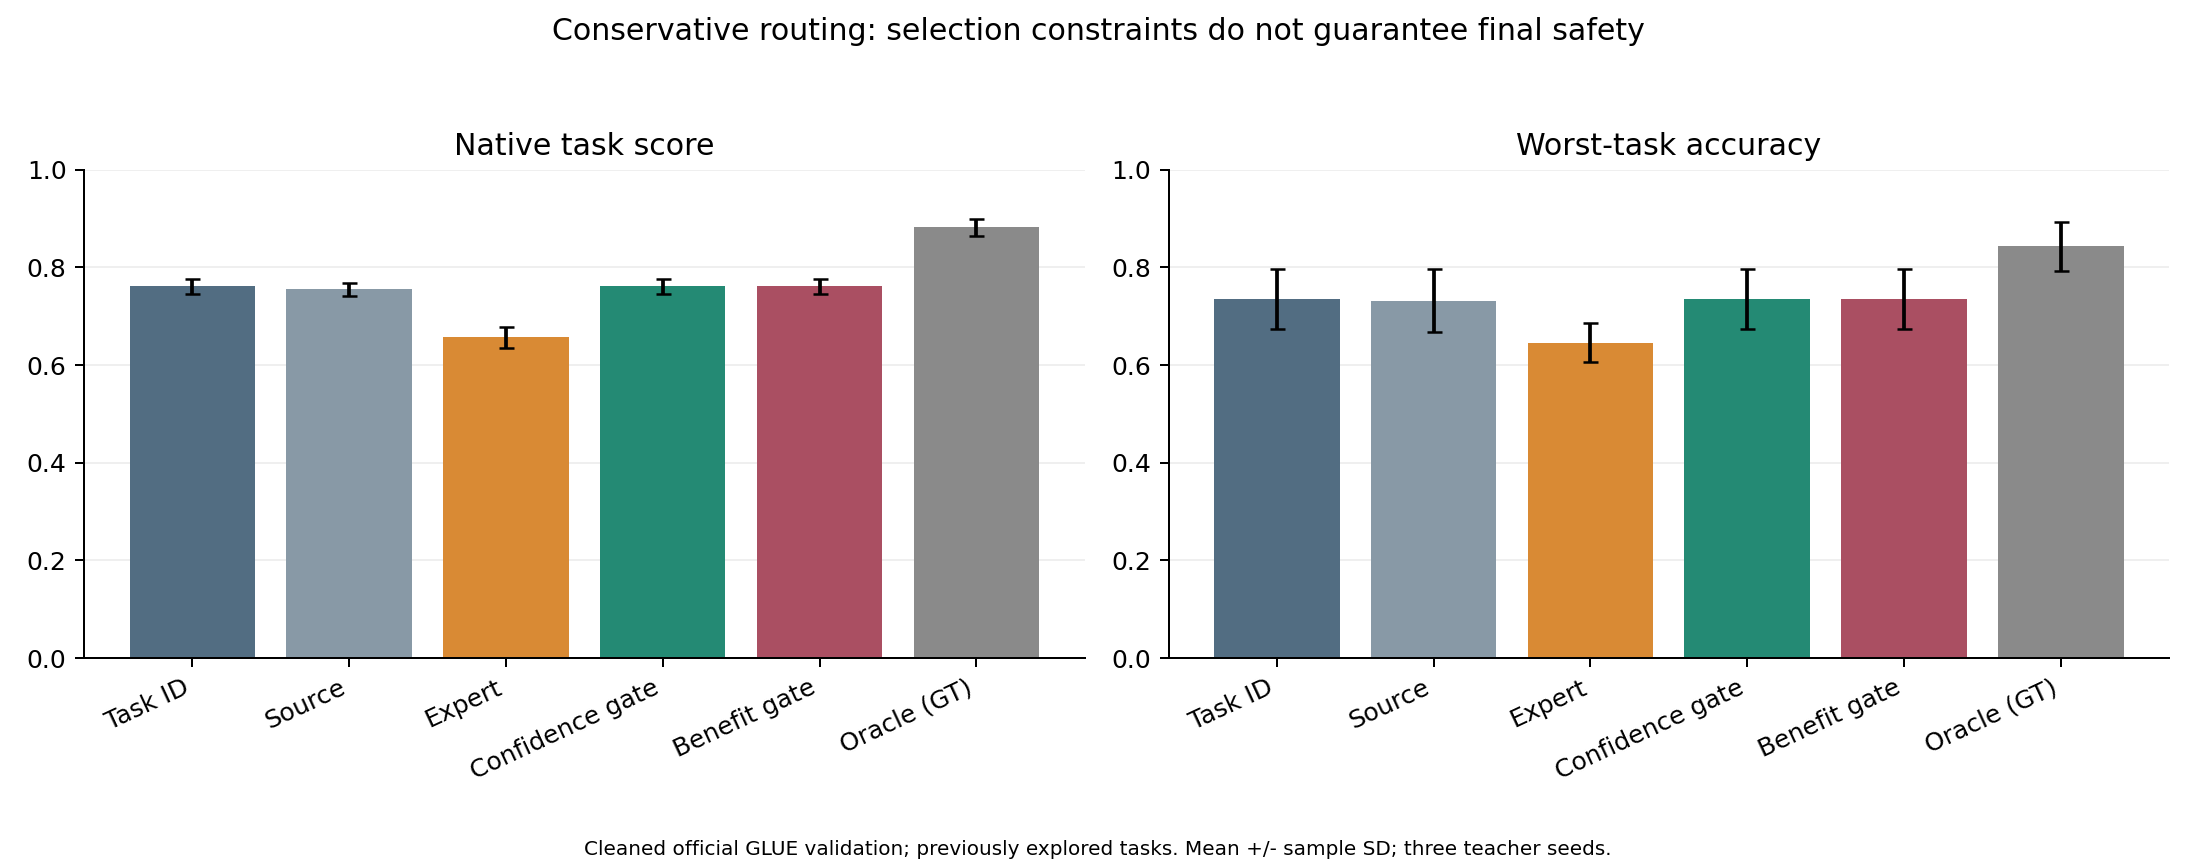
\includegraphics[width=\linewidth]{../artifacts/robustness-v2-2026-11-11/official-routing.png}
\caption{Actual final quality after conservative selection. A selection floor is not a final guarantee. Oracle uses final GT and is an analysis-only ceiling in this binary-task protocol.}
\end{figure}

\section{Deployment and external-transfer diagnostics}
\subsection{Measured cost of the current implementation}
An A100-SXM4-40GB benchmark uses fixed synthetic inputs, FP32, explicit CUDA synchronization, five warm-up calls and three rounds of 30 timed calls per shape/method. It includes base-feature extraction, CPU routing and state changes, and excludes model loading, tokenization, input transfer, and one-time materialization. These repeats are timing trials, not training seeds.

\begin{table}[H]\centering\small
\caption{Recorded implementation cost, batch one and 128 tokens. This benchmark uses the older seed-42 bank; it is separate from the v3 task-quality experiment.}
\begin{tabular}{lrr}\toprule
Implementation & Median latency (ms) & Peak allocated (GiB)\\\midrule
Individual materialized &23.459&1.940\\
Layer-KL materialized &23.375&1.940\\
Router, CPU dense-delta switch &98.589&1.940\\
Router, GPU dense-delta cache &48.971&2.350\\\bottomrule
\end{tabular}\end{table}

Static materialization has approximately the same single-backbone-forward cost as individual. Small submillisecond differences are not evidence of acceleration. Routing needs one base pass plus one forward for each distinct expert group in a batch; it is not always exactly two forwards. GPU caching reduces this implementation's transfer overhead but stores 336 MiB of dense deltas plus an 84 MiB zero-state copy. These costs are implementation-specific and do not characterize an optimized LoRA serving engine.

The new expert router's L4 quality and L4 serving latency have not been jointly benchmarked. We therefore do not combine its accuracy with historical A100 milliseconds to claim a measured Pareto improvement. The extra feature pass and expert grouping remain structural considerations.

One FP32 base has approximately 1.840 GiB of parameter payload. Four adapter directories total approximately 8.329 MiB, including their heads/configuration. Ninety-seven trained scalars are extra fitting parameters, not the entire deployment footprint. Comparing with four duplicated full backbones would exaggerate the storage saving relative to the actual shared-base bank.

\subsection{Source cues and out-of-domain failures}
A frozen earlier source router recognized 97.27\% of 512 validation sources. Removing explicit field headers reduced this to 93.75\%; uniform headers gave 95.12\%. Titles contribute, but sentence structure, length, and dataset style remain possible cues. The edit changes positions and length and does not isolate every source confound.

An earlier fixed transfer check evaluated 512 IMDb and 512 PAWS examples per method, with three protocol-v2 training seeds and no target tuning. \begin{table}[H]\centering\small
\caption{Historical protocol-v2 fixed transfer check: accuracy mean and sample SD across three training seeds; 512 examples per target.}
\begin{tabular}{lrr}\toprule
Method & IMDb & PAWS\\\midrule
Individual & 0.7090 $\pm$ 0.0237 & 0.4147 $\pm$ 0.0011\\
Average & 0.6758 $\pm$ 0.0276 & 0.4258 $\pm$ 0.0135\\
Uniform gain 2 & 0.7116 $\pm$ 0.0118 & 0.4316 $\pm$ 0.0220\\
Layer CE & 0.7051 $\pm$ 0.0198 & 0.4167 $\pm$ 0.0074\\
Layer KL (teacher-selected) & 0.6953 $\pm$ 0.0237 & 0.4167 $\pm$ 0.0041\\
\bottomrule\end{tabular}\end{table}

IMDb has substantial truncation at the 128-token limit; approximately 87\% of those samples exceed it. PAWS methods, including individual, fall below the subset majority-class accuracy of 59.375\%. These results do not establish robust transfer and cannot isolate merging as the sole cause. They involve earlier teachers, so they are not presented as new-v3 OOD measurements.

\section{Discussion and limitations}
The proposal's broad hypothesis contains distinct claims: similarity as a safety predictor, functional targets as a fitting signal, and dynamic routing as a useful serving mechanism. A successful implementation or high source-recognition score does not jointly establish these claims. The fixed v3 experiment supports learning a small static merge under calibration access, while its CE/KL control narrows the interpretation of that gain. \DiscussionExtension

The strongest practical reference is often task-ID selection because the evaluation already knows the head. Static merging can simplify weight-state management, but it incurs a task-quality gap and offers limited total-storage savings for a small shared-base bank. Routing must justify its quality gain against the extra feature pass, expert grouping, and fitting information. The oracle clarifies what this bank could achieve with impossible knowledge; it does not demonstrate that the corresponding choices can be learned from the available features.

This is a small-backbone, four-task case study. The tasks are binary, share a fixed split, and have been explored before. Exact-tuple deduplication has a limited scope. Three training seeds do not support broad statistical conclusions. The selection labels make the pipeline supervised; stronger data-free or unknown-task claims require different protocols. We do not test every adapted-module subset, model family, LoRA rank, or modern alignment baseline. CE+$H$ weight one and the energy floor are fixed design choices, not established optima. The shuffled control tests input pairing and leaves broader style confounding possible.

Our course project's Part 1 studies CSA. It informs interest in structured representations and explicit storage budgets, but current Part 2 code does not apply CSA mode projections to LoRA updates. The connection is conceptual rather than an implemented CSA-to-LLM transfer. A full proposal-aligned report can therefore state both what was implemented and which original expectations remain unsupported.

\section{Conclusion}
We implemented a reproducible, task-aware LoRA merging study with weight-space baselines, supervised and functional coefficient objectives, explicit data boundaries, and routing diagnostics. The v3 mean native task scores are 0.7695 for individual, 0.7132 for layer CE, 0.6987 for layer KL, and 0.6146 for our TIES variant. Learned coefficients recover part of the averaging loss, while teacher-output KL has no average advantage over its matched-capacity CE control. \ConclusionExtension\ \ConclusionVtwo\ The defensible outcome is evidence about the utility and failure conditions of functional proxies in this setting, together with measured implementation trade-offs and a reproducible pipeline.

\appendix
\section{Reproducibility and implementation checks}
After a browser interruption, the earlier temporary VM was reclaimed before complete result download. We recovered intact CSV and figure records from the partial archive, verified their CRC and original manifest hashes, and reran the frozen extension on 11 November from the checksummed 12-teacher backup. The final package contains the full rerun predictions and a comparison with recovered metrics. This repeats the same three training seeds and does not increase the number of independent replications to six.

Exact model/data revisions and partition checksum are recorded below.
\begin{quote}\footnotesize
Model: \texttt{060db6499f32faf8b98477b0a26969ef7d8b9987}\\
GLUE: \texttt{bcdcba79d07bc864c1c254ccfcedcce55bcc9a8c}\\
Partition SHA256:\\
\texttt{526c3ae3aefebf36f651c0518d4a69b1c51d8c2e9d5145063f791b0b363386eb}
\end{quote}
The code records environment versions, ID lists, selected checkpoints, coefficients, gains, source SHA, and prediction artifacts. Model computation runs in Colab; generated sources and figures accompany this report.

The pinned research stack uses a system-site-packages virtual environment. Inherited optional packages generated pip dependency-conflict warnings; those unrelated packages are not used here. We report successful research-module checks and actual imports rather than a globally clean pip check.

Checks cover merge arithmetic, masked pooling, a shuffled target's lack of fixed points, oracle invariance to additive logit shifts, nonzero coefficient gradients, no gradients on frozen parameters, low-rank/dense logit parity, task-ID/individual metric parity, and split permissions. The extension additionally audits saved predictions independently of model fitting. Versioned results preserve exploratory stages instead of overwriting earlier outcomes.

The v3 checkpoint backup contains 12 adapters and 131 verified files. Restoration was tested into a new directory with relocated manifest paths; corrupt SHA, unsafe archive paths, and overwriting an existing directory were rejected. The shared base/tokenizer are obtained separately at pinned Hub revisions. The runtime connection client is closed after exports have been downloaded and verified; closing it is distinct from releasing the cloud VM.

The follow-up checks cover scalar-weight overrides, fallback behavior without feature extraction, selection rejection and tie rules, label-blind content filtering, stored classifier probabilities, selection-only lambda choice, cached split/label alignment, and reload parity of the selected gates. Saved official predictions are audited independently for every method and task. All experiments use frozen teacher banks; feature caches and raw text stay outside the published evidence archive.

\subsection{Execution overview}
\small
\begin{verbatim}
python code/run_independent_study.py --output outputs/new-v3
python code/independent_baselines.py --study outputs/new-v3
python code/activation_extension.py --study outputs/new-v3 \
  --plan configs/activation-strengthening-v1.json \
  --output outputs/new-extension
\end{verbatim}
\normalsize
Output directories must be new. The extension requires the matching locked manifest and teacher bank. Compiler commands and data-generation sources are provided in the package README. Group scheduling, formal submission requirements, and teammate access are administrative checks separate from scientific completion.

\begin{thebibliography}{11}\small
\bibitem{lora} E. J. Hu et al. \emph{LoRA: Low-Rank Adaptation of Large Language Models}. 2021. \url{https://arxiv.org/abs/2106.09685}.
\bibitem{ta} G. Ilharco et al. \emph{Editing Models with Task Arithmetic}. ICLR 2023. \url{https://arxiv.org/abs/2212.04089}.
\bibitem{ties} P. Yadav et al. \emph{TIES-Merging: Resolving Interference When Merging Models}. 2023. \url{https://arxiv.org/abs/2306.01708}.
\bibitem{dare} L. Yu et al. \emph{Language Models are Super Mario: Absorbing Abilities from Homologous Models as a Free Lunch}. ICML 2024. \url{https://arxiv.org/abs/2311.03099}.
\bibitem{regmean} X. Jin et al. \emph{Dataless Knowledge Fusion by Merging Weights of Language Models}. ICLR 2023; arXiv version 6 consulted. \url{https://arxiv.org/abs/2212.09849}.
\bibitem{adamerge} E. Yang et al. \emph{AdaMerging: Adaptive Model Merging for Multi-Task Learning}. ICLR 2024. \url{https://arxiv.org/abs/2310.02575}.
\bibitem{knots} G. Stoica et al. \emph{Model Merging with SVD to Tie the Knots}. 2024 preprint / ICLR 2025. \url{https://arxiv.org/abs/2410.19735}.
\bibitem{fitnets} A. Romero et al. \emph{FitNets: Hints for Thin Deep Nets}. 2015. \url{https://arxiv.org/abs/1412.6550}.
\bibitem{glue} A. Wang et al. \emph{GLUE: A Multi-Task Benchmark and Analysis Platform for Natural Language Understanding}. 2018. \url{https://arxiv.org/abs/1804.07461}.
\bibitem{qwen} Qwen Team. \emph{Qwen2.5 Technical Report}. 2024; revised 2025. \url{https://arxiv.org/abs/2412.15115}.
\end{thebibliography}
\end{document}
